In this part, we switch to Matlab in order to design our parameters for the PD controller with the help of necessary tools. To define our transfer function there, we first initialize our parameters. Figure \ref{fig:init} shows our initialization part at the beginning of our script.

\begin{figure}[H]
    \centering
    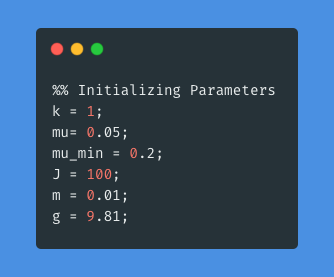
\includegraphics[width=0.7\textwidth]{images/initalization.png}
    \caption{Parameter Initialization}
    \label{fig:init}
\end{figure}

Once these are defined, we then create our plant by defining the numerator and denominator and passing them to tf() function. The obtained transfer function will be fed into rlocus() and sisotool() methods to be manipulated further. As can be seen from Figure \ref{fig:plant_ss}.

\begin{figure}[H]
    \centering
    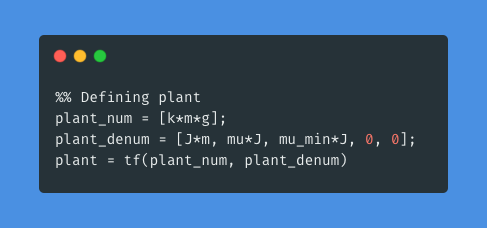
\includegraphics[width=0.9\textwidth]{images/plant_def.png}
    \caption{Creating the Plant}
    \label{fig:plant_ss}
\end{figure}
\newpage
When we see the \textit{}{Root Locus plot} of this plant, we get the following figure. As can be seen, this system is not stable since it has 2 roots on the imaginary axis. Our aim is to introduce another \textit{zero} to the system in order to obtain a configuration where all roots have negative real parts.

\begin{figure}[H]
    \centering
    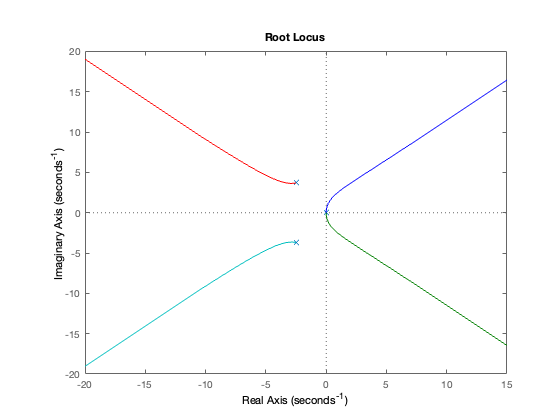
\includegraphics[width=0.7\textwidth]{images/initial_rlocus.png}
    \caption{Root Locus Plot}
    \label{fig:initial_locus}
\end{figure}


Furthermore, the step response plot obtained from the sisotool() GUI confirms that the system is not stable. Figure \ref{fig:siso1} below shows this behavior.

\begin{figure}[H]
    \centering
    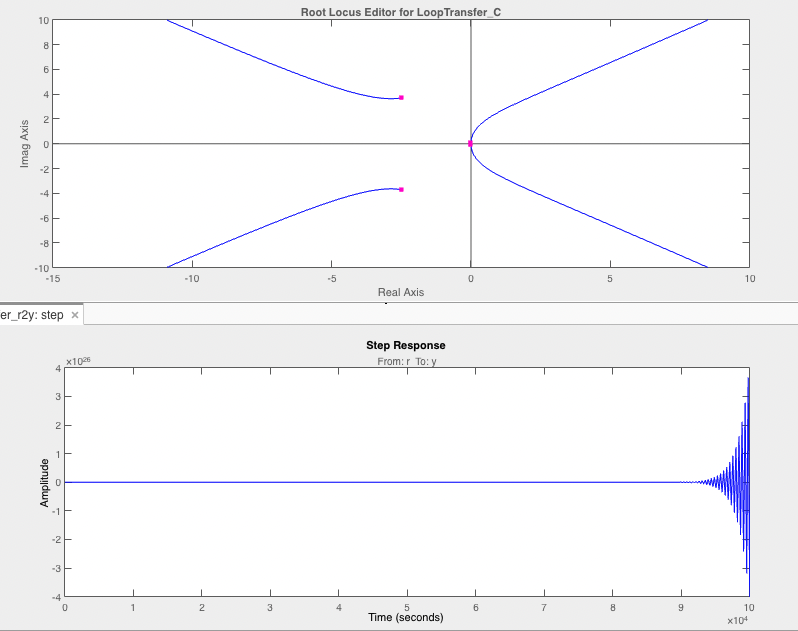
\includegraphics[width=0.7\textwidth]{images/siso1.png}
    \caption{Sisotool Screen}
    \label{fig:siso1}
\end{figure}

\newpage

The PD controller allows us to \textbf{introduce a new zero} to our system. This zero can be placed strategically in order to manipulate the \textit{Root Locus plot} and obtain a configuration where all the root have negative real parts. There are 3 main places that our new zero can be placed. They are as follows:



\begin{itemize}
    \item To the right of all poles
    \item Between the poles on the imaginary axis and the negative poles
    \item To the left of all poles
    
\end{itemize}

\subsection{Zero at the Positive Side}
When the zero is added to first mentioned location, this system does not benefit and continues to be unstable. A sample plot that shows this behavior is shown in Figure \ref{fig:zeroright} below.

\begin{figure}[H]
    \centering
    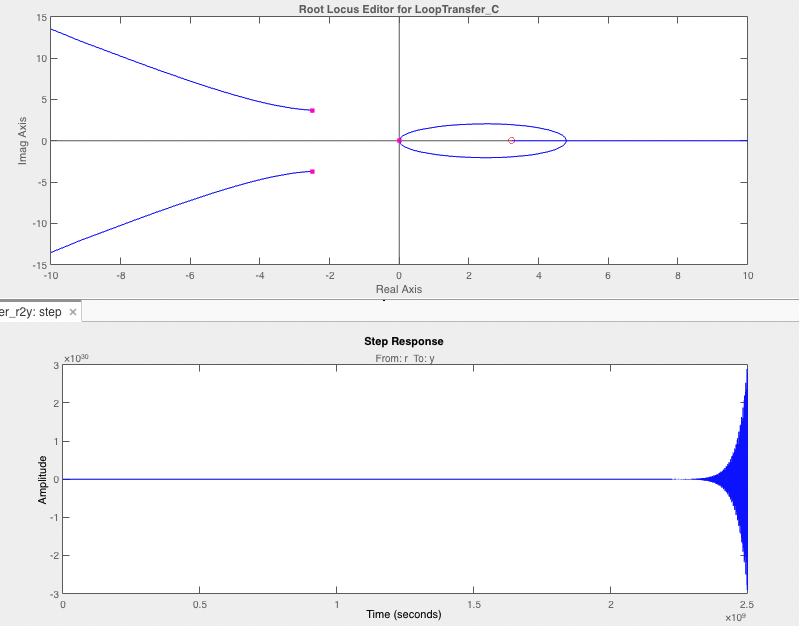
\includegraphics[width=0.8\textwidth]{images/zero_positive.png}
    \caption{Zero added to the positive real part}
    \label{fig:zeroright}
\end{figure}


\subsection{Zero Between to the Pole Pairs}
The second placement option for our zero actually allows a stable system. When the zero is placed between the two pole pairs, we obtain the option to select our $K_d$ and $K_p$ values to stabilize the system. A figure showing this behavior is given below on Figure \ref{fig:zerobetween}. Although there is significant overshoot, this configuration can be stable and the design parameters can and will be further optimized throughout this report.

\begin{figure}[H]
    \centering
    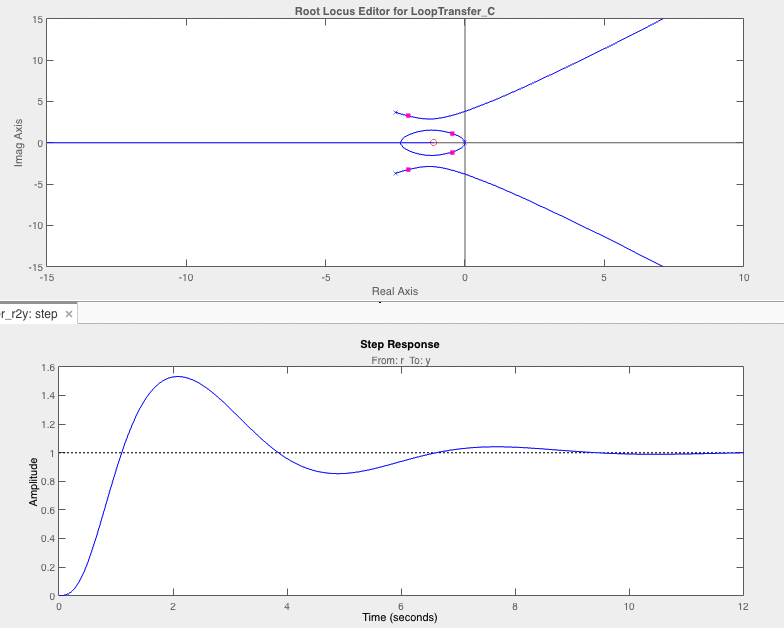
\includegraphics[width=0.6\textwidth]{images/zero_between.png}
    \caption{Zero added between the two pairs}
    \label{fig:zerobetween}
\end{figure}


\subsection{Zero to the Left of Poles}

This placement condition was first thought to not allow any stable configurations. However, it is then realized that there exists a small region to the left of the negative poles where the system in fact, can be stable. \\

A sample configuration for the unstable case is shown below.

\begin{figure}[H]
    \centering
    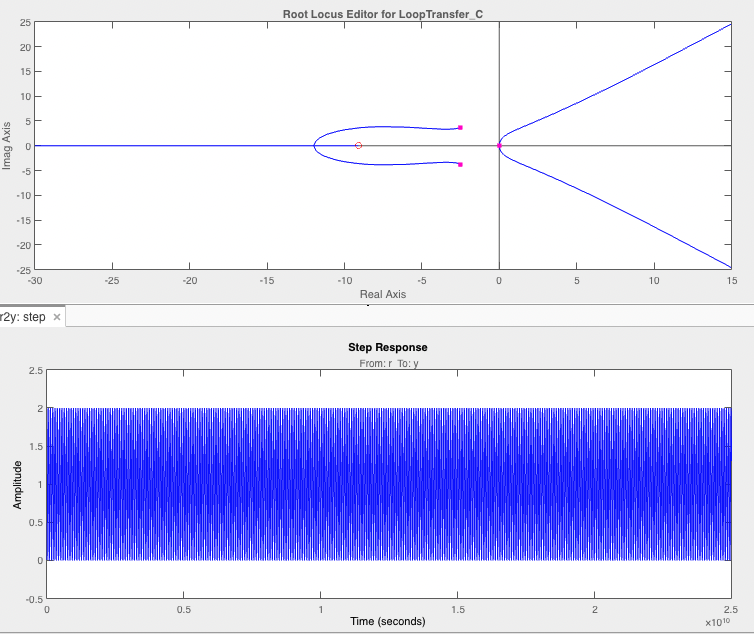
\includegraphics[width=0.8\textwidth]{images/zero_right.png}
    \caption{Zero added to the left the two pairs}
    \label{fig:zerobetween}
\end{figure}

\newpage
\subsection{Optimizing the Parameters }
\subsubsection{Smaller Overshoot}
We continued by optimizing different design parameters individually. We also used the PID tuning tools to help us with this task. Our first optimization was keeping the overshoot at the minimum. This was observed when the zero value was close to the imaginary axis. This system is shown on the Figure \ref{fig:overs} below.

\begin{figure}[H]
    \centering
    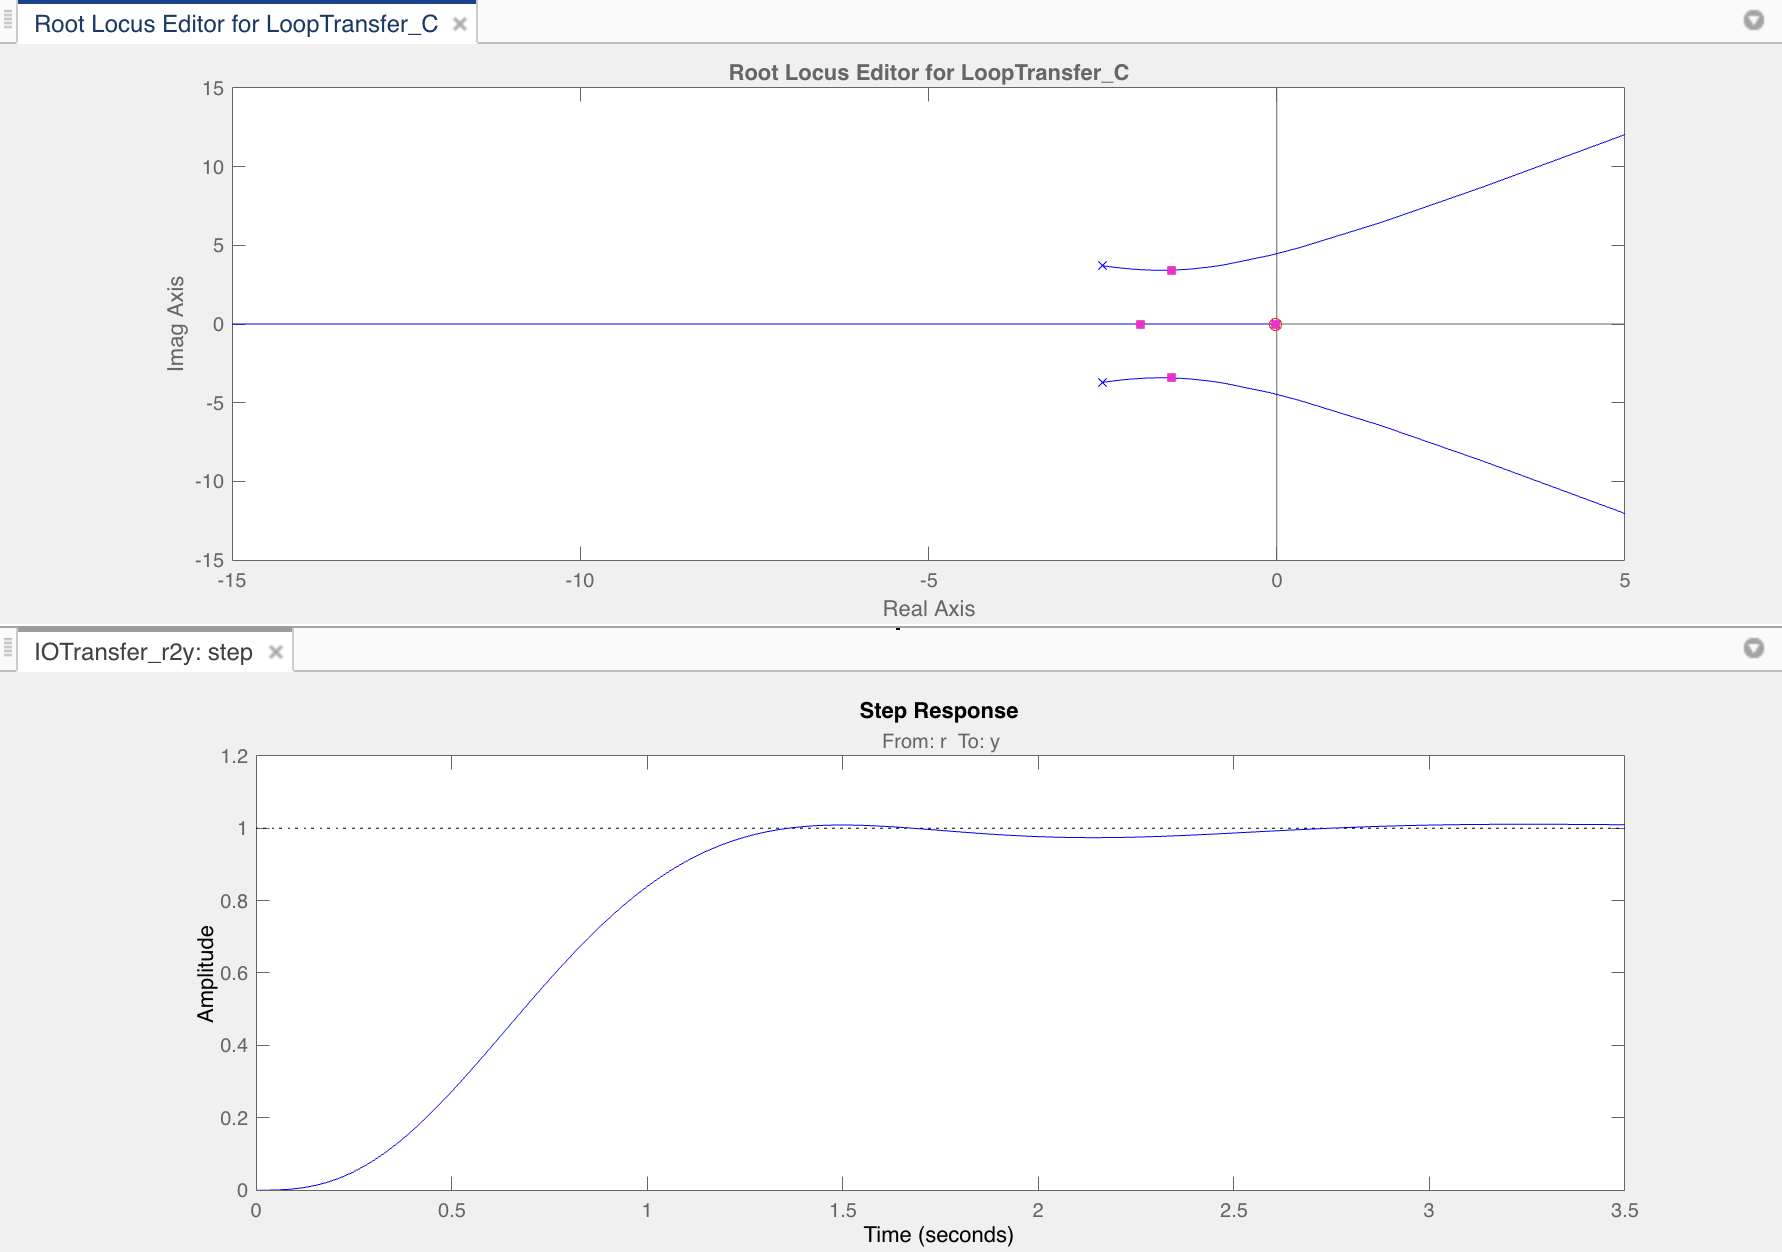
\includegraphics[width=0.9\textwidth]{images/minimum overshoot.png}
    \caption{System with small overshoot}
    \label{fig:overs}
\end{figure}

This system has a slower response time but it is very robust. The equation of the controller that corresponds to this system is as follows:
\begin{equation}
    C(s) = 3.27 * (1 + 86s)
\end{equation}


\subsubsection{Aggressive but Oscillatory Configuration}
We then optimized our system to have a more aggressive response. This, as expected, resulted in a oscillatory configuration that overshoots significantly more than the previous configuration. The response of this system is shown below:
\begin{figure}[H]
    \centering
    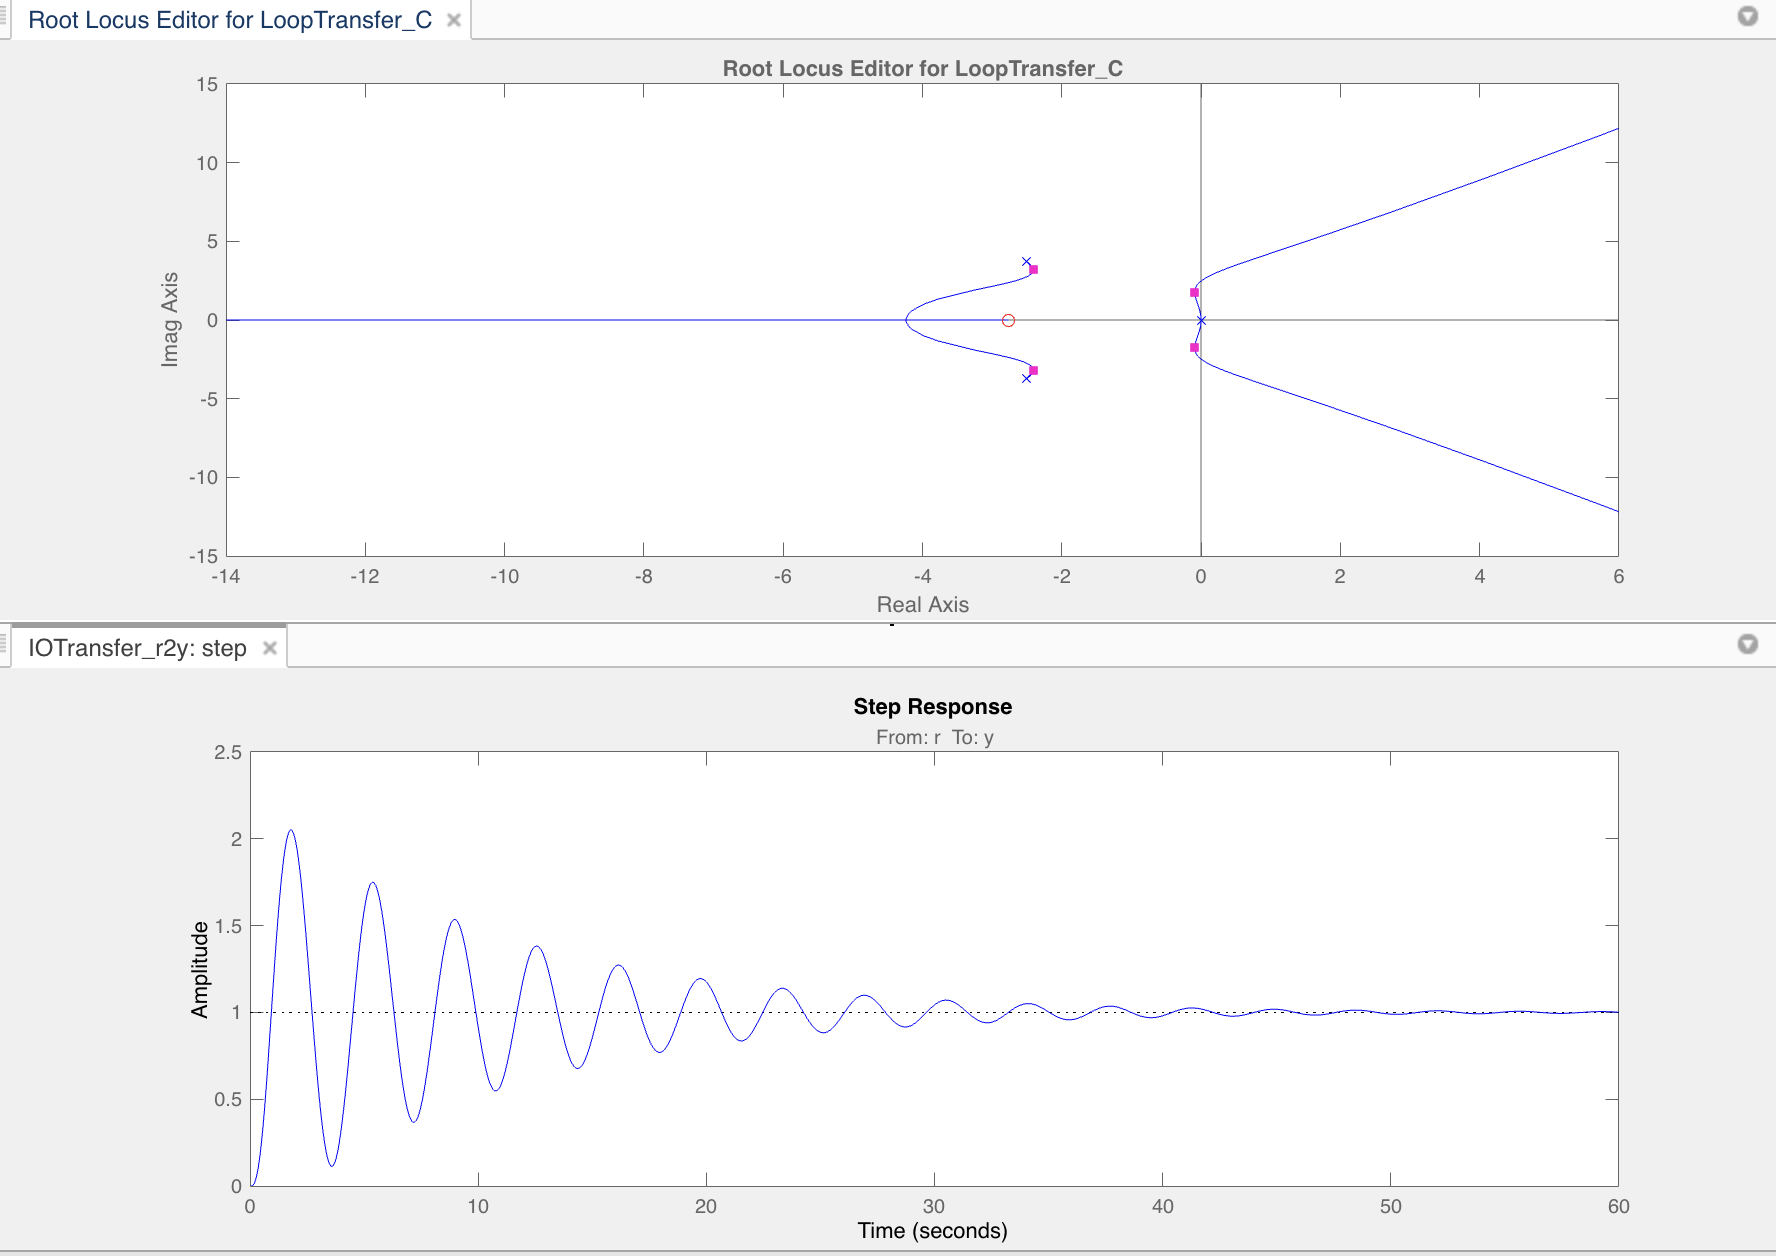
\includegraphics[width=0.9\textwidth]{images/oscillatory.png}
    \caption{A more aggressive system}
    \label{fig:agg}
\end{figure}

Note that the zero value is to the left of all poles in this configuration. Also, the controller that corresponds to this system is shown below:
\begin{equation}
        C(s) = 502 * (1 + 36s)
\end{equation}

\subsubsection{Final Configuration}
With our experience from the previous systems, we then continued with a new controller that we think is the best for our use in this project. It has very little overshoot, is fairly responsive and robust. A sample output of this configuration is shown below.


\begin{figure}[H]
    \centering
    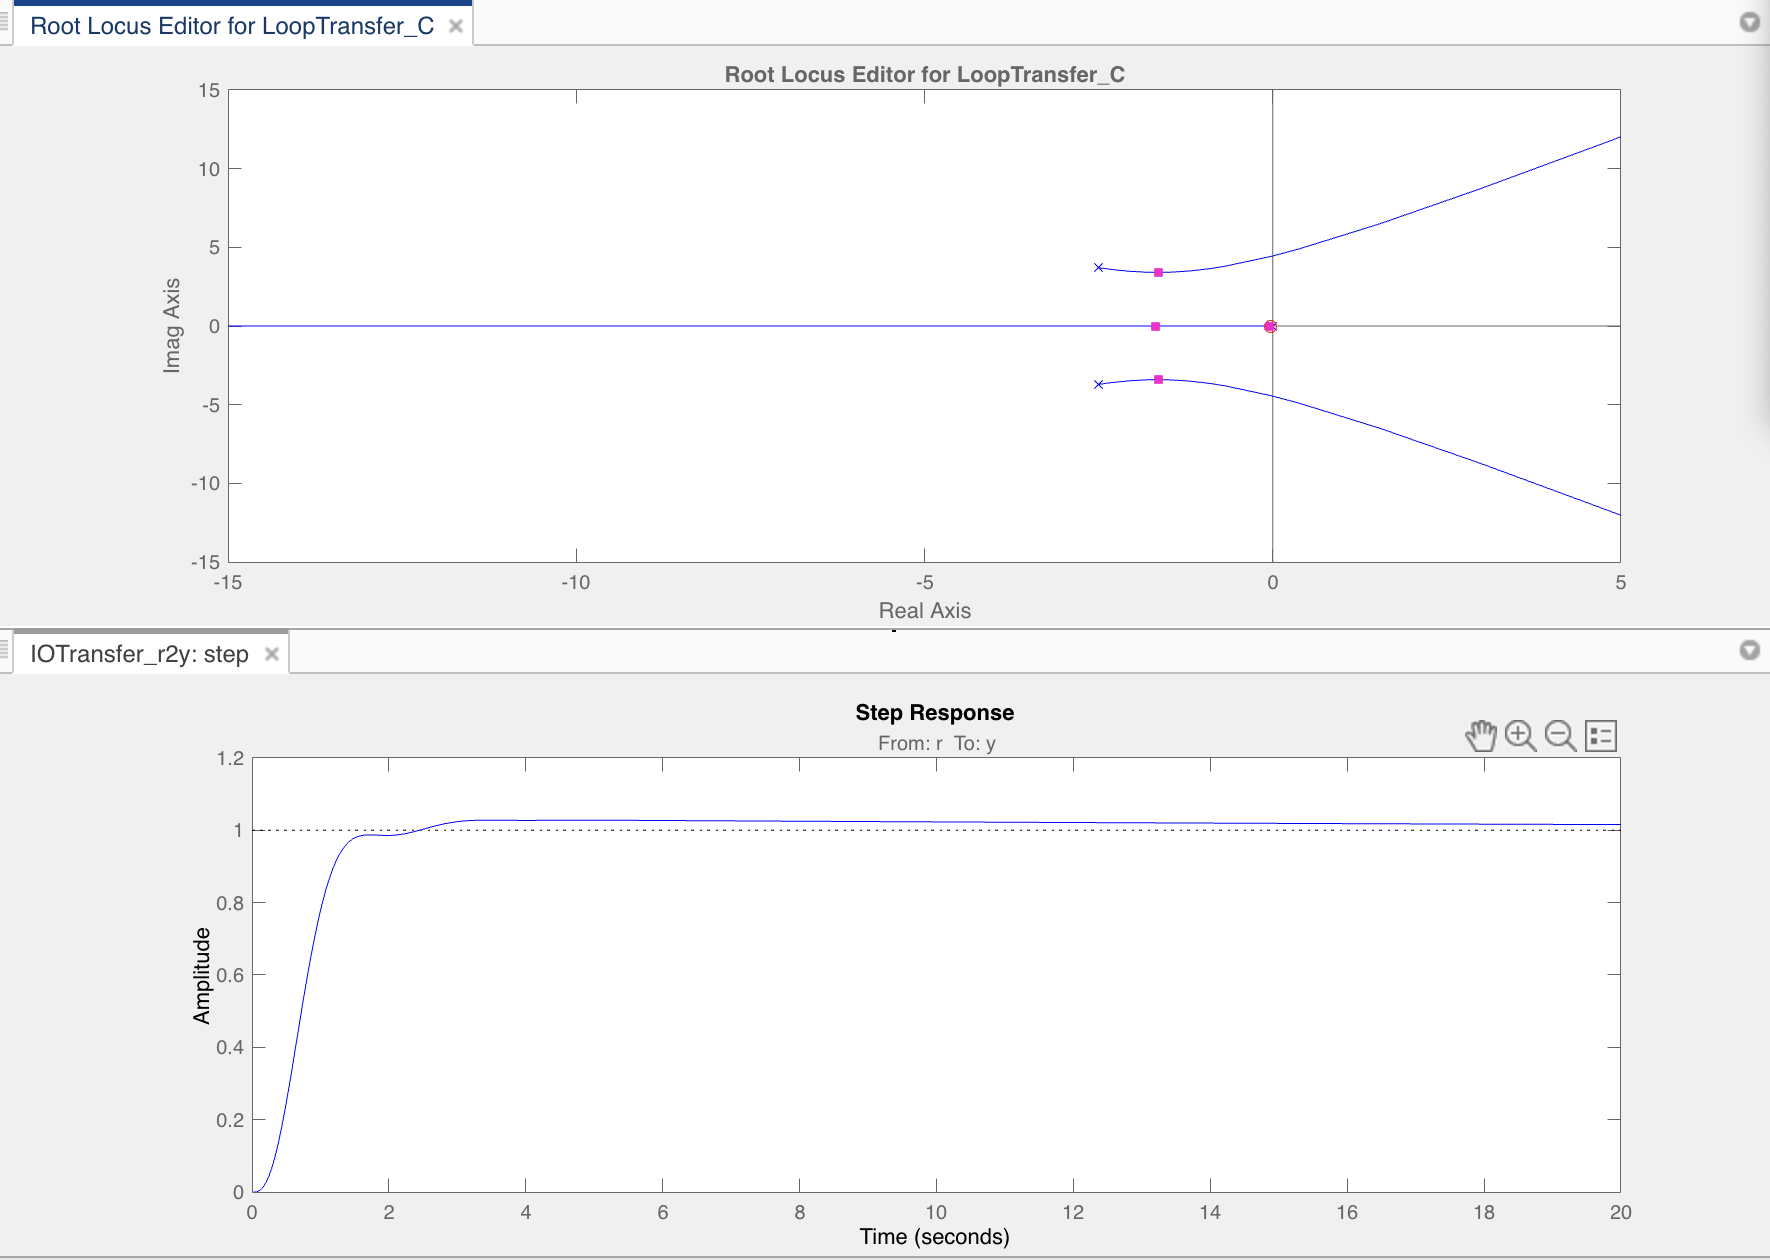
\includegraphics[width=0.9\textwidth]{images/fisek_response.png}
    \caption{Proposed system}
    \label{fig:fisek}
\end{figure}

The controller that corresponds to this system is shown below:

\begin{equation}
        C(s) = 9.75 * (1 + 26)
\end{equation}


\section{Conclusion}


In conclusion, we tried different parameters for our controller and deduced that any \textbf{zero} that is introduced by the PD controller that is between 0 and -3.5 gives the opportunity to stabilize the system. However, the 3 controllers we have proposed work the best for our case.